% ============================================================
%  CINF104 – Proyecto 1: Predicción GRD
%  IEEE Access template
%  Universidad Andrés Bello – 2026
% ============================================================
\documentclass{IEEEtran}

% ── Packages ────────────────────────────────────────────────
\usepackage[T1]{fontenc}
\usepackage[utf8]{inputenc}
\usepackage{cite}
\usepackage{amsmath,amssymb}
\usepackage{graphicx}
\usepackage{booktabs}
\usepackage{hyperref}
\usepackage{url}
\usepackage{float}
\usepackage{multirow}
\usepackage{array}

\hypersetup{
  colorlinks=true,
  linkcolor=blue,
  citecolor=blue,
  urlcolor=blue
}

% ── Title / Authors ─────────────────────────────────────────
\title{GRD Prediction in Clinical Data Using Machine Learning:\\
A Multi-class Classification Approach for Hospital El Pino}

\author{
  \IEEEauthorblockN{Cristóbal Flores Villegas,
                    Benjamin Peña Díaz,
                    Matías Muñoz Parraguirre,
                    Francisco Morales Díaz.
                   }
                   
  \IEEEauthorblockA{
    \textit{Escuela de Informática, Ingeniería Civil Informática}\\
    \textit{Universidad Andrés Bello}\\
    Santiago, Chile \\
    \texttt{CINF104 – Aprendizaje de Máquinas, 2026}
  }
}

\begin{document}
\maketitle

% ── Abstract ────────────────────────────────────────────────
\begin{abstract}
Diagnosis-Related Groups (DRGs) are a patient classification system
widely used in healthcare for hospital resource planning and billing.
Manually assigning the correct DRG is time-consuming and error-prone.
This paper presents a machine learning pipeline for automatic DRG
prediction from clinical data of Hospital El Pino, Chile.
We explore three classification approaches—Random Forest (RF),
LightGBM, and a Multi-Layer Perceptron (MLP)—on a dataset of
14{,}561 patients described by ICD diagnostic codes, procedure codes,
age, and sex.
Because the 526 original DRG classes exhibit a heavy long-tail
distribution (76 singletons, 199 classes with fewer than 5 examples),
we adopt a \emph{long-tail} target strategy that retains the 229 most
frequent specific DRGs and groups the remainder into an \textsc{Others}
class, yielding 230 balanced classes.
Features are built via multi-hot encoding over the top-200 diagnostic
codes and top-83 procedure codes, enriched with numeric features
(age, diagnosis count, procedure count, sex).
The MLP achieves the best performance with a validation accuracy of
63.8\%, a macro-F1 of 42.0\%, and a top-3 accuracy of 84.2\%,
demonstrating that deep learning outperforms tree-based baselines
on this heavily imbalanced multi-class problem.
\end{abstract}

\begin{IEEEkeywords}
DRG prediction, hospital classification, ICD codes, multi-class
classification, deep learning, MLP, LightGBM, Random Forest,
long-tail distribution, clinical informatics
\end{IEEEkeywords}

% ── 1. Introduction ─────────────────────────────────────────
\section{Introduction}

Diagnosis-Related Groups (DRGs) constitute a patient classification
framework designed to standardise hospital reimbursement and resource
allocation~\cite{fetter1980drg}.
In Chile, the \emph{Informe de Referencia GRD} (IR-GRD) classifies each
inpatient episode into one of hundreds of groups based on the principal
diagnosis, secondary diagnoses, performed procedures, age, and sex.
Correct DRG assignment is critical: coding errors lead to under- or
over-billing, biased epidemiological statistics, and misallocation
of hospital resources~\cite{topol2019highperformance}.

Despite its importance, DRG coding in many Chilean public hospitals
is still performed manually by trained registrars working from medical
records written in natural language.
This process is slow, subjective, and difficult to audit.
An automated prediction system would reduce coding time,
flag potential errors, and serve as a decision-support tool
for clinical staff.

Recent advances in machine learning (ML) and natural language
processing (NLP) have demonstrated strong performance on medical
coding tasks~\cite{mullenbach2018explainable}.  However, most
published systems target ICD coding rather than DRG coding, and
few focus on the Chilean IR-GRD nomenclature or on small-to-medium
hospital datasets.

This work makes the following contributions:
\begin{itemize}
  \item We analyse the hierarchical structure of the Chilean IR-GRD
        code system and propose a \emph{long-tail} target strategy
        to handle the extreme class imbalance.
  \item We design and evaluate a full ML pipeline—from raw ICD
        codes to trained classifiers—comparing three families of
        models: Random Forest, gradient boosting (LightGBM), and
        a deep MLP.
  \item We report accuracy, macro-F1, weighted-F1, and top-3
        accuracy on a real-world dataset of 14{,}561 patients from
        Hospital El Pino, Chile.
\end{itemize}

% ── 2. Related Work ─────────────────────────────────────────
\section{Related Work}

\subsection{Automated ICD and DRG Coding}
Mullenbach et al.~\cite{mullenbach2018explainable} proposed CAML, a
convolutional attention model for multi-label ICD coding achieving
AUC above 0.90 on MIMIC-III discharge summaries.
Huang et al.~\cite{huang2019clinicalbert} showed that clinical
BERT variants substantially improve code prediction when trained on
in-domain text.
In the DRG prediction domain, Raju et al.~\cite{raju2021drg}
trained gradient-boosted trees on structured EHR features,
reaching 72\% accuracy for Major Diagnostic Category (MDC)
prediction, a coarser granularity than individual DRGs.

\subsection{Handling Long-Tail Distributions in Medical Data}
Class imbalance is endemic in clinical datasets.
Strategies include oversampling (SMOTE)~\cite{chawla2002smote},
cost-sensitive learning, and hierarchical classification where
coarse-to-fine predictions are combined~\cite{chen2019hiagm}.
We adopt a pragmatic long-tail approach: DRGs with fewer than
10 training examples are grouped into an \textsc{Others} class,
reducing noise while preserving specificity for common episodes.

\subsection{Feature Engineering for Structured Clinical Data}
Purushotham et al.~\cite{purushotham2018benchmarking} benchmark
multiple ML methods on MIMIC-III clinical tasks, finding that
ensemble methods and simple neural networks perform comparably
when features are carefully engineered from structured data.
This supports our choice of multi-hot ICD encoding as a feature.

% ── 3. Objective ────────────────────────────────────────────
\section{Objective}

The primary objective of this study is to build and evaluate a
machine learning model that automatically predicts the Chilean
IR-GRD code of a patient given the following structured inputs:
principal and secondary ICD diagnostic codes (up to 35),
procedure codes (up to 30), age, and sex.
Secondary objectives include:
\begin{enumerate}
  \item Identifying the appropriate target granularity for the
        DRG prediction problem.
  \item Comparing the performance of tree-based and neural network
        architectures under heavy class imbalance.
  \item Producing a reproducible, open-source pipeline suitable
        for integration into hospital information systems.
\end{enumerate}

% ── 4. Methodology ──────────────────────────────────────────
\section{Methodology}
\label{sec:method}

\subsection{Dataset Description}

The dataset was provided by Hospital El Pino, a public secondary-care
hospital located in San Bernardo, Chile.
It contains \textbf{14{,}561} inpatient episodes recorded in a
single fiscal year, each described by 68 columns:
\begin{itemize}
  \item \textit{Diagnóstico principal} and up to 34 secondary
        diagnoses, encoded as combined ICD code + description
        strings (e.g., \texttt{A41.8 - Otras septicemias}).
  \item Up to 30 procedure codes similarly formatted.
  \item \textit{Edad en años}: patient age in years (integer, 0–121).
  \item \textit{Sexo}: patient sex (Mujer / Hombre).
  \item \textit{GRD}: target label, formatted as
        \texttt{<6-digit-code> - <description>}.
\end{itemize}

The dataset contains \textbf{no missing values} in any of the four
key columns (principal diagnosis, age, sex, GRD).
Mean patient age is 39.4 years (std 24.7), and the sex distribution
is 66\% female – 34\% male, reflecting Hospital El Pino's high
volume of obstetric episodes.
On average each patient has all 35 diagnosis slots filled and all 30
procedure slots filled, indicating uniform completeness in data
collection.

\subsection{Target Granularity Analysis}

The IR-GRD code is a 6-digit number with a hierarchical structure:
digit 1 encodes episode type (1=Medical/MH, 2=Surgical/PH),
digits 2–3 encode the Major Diagnostic Category (CDM, 22 classes),
and subsequent digits encode the specific DRG and severity level.

We analysed five levels of granularity, summarised in
Table~\ref{tab:granularity}.
The full DRG level presents 526 classes with 76 singletons
(Gini impurity 0.733) and requires 119 of them to cover 80\%
of patients—rendering direct prediction impractical without
aggregation.
CDM (22 classes) is tractable but too coarse for clinical utility.
We therefore adopt a \emph{long-tail} strategy at the full DRG
level: DRGs with $\geq 10$ training examples (229 classes, covering
92.4\% of patients) are kept as-is; the remaining are mapped to
\textsc{Others}, yielding \textbf{230} prediction targets.

\begin{table}[H]
  \centering
  \caption{GRD Granularity Levels}
  \label{tab:granularity}
  \begin{tabular}{lrrrr}
    \toprule
    Level & Classes & Singletons & K@80\% & Gini \\
    \midrule
    grd\_full  & 526 & 76 & 119 & 0.733 \\
    grd\_base  & 69  & 5  & 18  & 0.709 \\
    grd\_cdm\_base & 37 & 1 & 13 & 0.617 \\
    cdm        & 22  & 0  & 11  & 0.477 \\
    tipo\_phmh & 3   & 0  & 2   & 0.311 \\
    \bottomrule
  \end{tabular}
\end{table}

\subsection{Feature Engineering}

\textbf{ICD Code Extraction.}
Each diagnosis/procedure string is parsed by splitting on
`` – '' and retaining the first 3 characters of the code
(Chapter-level ICD-10/ICD-9), normalising free-text to a
categorical vocabulary.

\textbf{Multi-hot Encoding.}
The top-200 most frequent 3-character diagnostic codes and the top-83
most frequent procedure codes are selected from the training set.
Each patient is represented as a binary vector of length $200+83=283$
indicating code presence.

\textbf{Numeric Features.}
Age (standardised), number of diagnoses, number of procedures, and
sex (binary) are appended, giving a final feature vector of
$\mathbf{287}$ dimensions per patient.

\textbf{Data Split.}
The dataset is split stratified by class label:
70\% train (10{,}192), 15\% validation (2{,}184), 15\% test (2{,}185).
Continuous features are standardised using a
\texttt{StandardScaler} fitted on the training partition only.

\subsection{Models}

\textbf{Random Forest (RF).}  A classic ensemble of 200 decision
trees (max depth 25, min samples per leaf 2) serves as the
interpretable baseline.  RF handles multi-class out of the box
via majority vote.

\textbf{LightGBM.}  A gradient-boosted decision tree framework
with 500 estimators, learning rate 0.05, and 63 leaves per tree.
Early stopping (patience 50) on validation loss prevents overfitting.
LightGBM is known to excel on tabular data~\cite{ke2017lightgbm}.

\textbf{MLP.}  A feedforward neural network with three hidden layers
(512–256–128 neurons), ReLU activations, Batch Normalisation,
and Dropout (0.4–0.3–0.2).  Trained with Adam ($lr{=}10^{-3}$),
sparse categorical cross-entropy loss, and EarlyStopping
(patience 10, monitoring validation accuracy).
The best checkpoint is restored at the end of training.

\subsection{Evaluation Metrics}

Given the extreme class imbalance (230 classes, 92.4\% in specific
DRGs), we report:
\begin{itemize}
  \item \textbf{Accuracy}: share of exactly correct predictions.
  \item \textbf{Macro-F1}: unweighted mean F1 across all classes,
        penalising poor performance on minority classes.
  \item \textbf{Weighted-F1}: F1 weighted by class support.
  \item \textbf{Top-3 Accuracy}: the ground-truth DRG appears among
        the three highest-probability predictions—relevant for
        decision-support scenarios.
\end{itemize}

% ── 5. EDA ──────────────────────────────────────────────────
\section{Exploratory Data Analysis}

\subsection{Data Quality and Outlier Analysis}

As shown in Table~\ref{tab:null}, the four key columns contain
zero missing values, indicating a high-quality, pre-curated
administrative dataset.
All 14{,}561 patients have a complete principal diagnosis, age,
sex, and GRD label.

\textbf{Age outliers.}
Using the interquartile range (IQR) method
($Q_1{=}23$, $Q_3{=}60$, $\mathrm{IQR}{=}37$,
upper fence $= 115.5$), only 1 record exceeds the fence
($<$0.01\% of data).
Two patients have ages above 100 years (one recorded as 121),
which may represent data-entry errors; however, given the
negligible proportion, these records were retained as-is
to avoid introducing bias.
Ages of zero (1{,}395 records, 9.6\%) correspond to
neonatal episodes and are clinically valid.

\textbf{GRD class outliers (long-tail).}
The target variable exhibits a severe long-tail distribution:
76 classes are \emph{singletons} (a single patient per class)
and 131 classes contain 2 or fewer patients.
These ultra-rare classes are statistically unlearnable and
constitute the primary source of label noise;
they are addressed in Section~\ref{sec:method} via the
long-tail aggregation strategy.

\textbf{Correctness.}
ICD codes appear in the expected format
(\texttt{AAA.B – Description}).
No invalid code patterns were detected after extraction.
The GRD codes conform to the 6-digit IR-GRD structure.

\begin{table}[H]
  \centering
  \caption{Missing Values in Key Columns}
  \label{tab:null}
  \begin{tabular}{lr}
    \toprule
    Column & Missing \\
    \midrule
    Principal Diagnosis & 0 \\
    Age (years)         & 0 \\
    Sex                 & 0 \\
    GRD                 & 0 \\
    \bottomrule
  \end{tabular}
\end{table}

\subsection{Descriptive Statistics}

\textbf{Patient demographics.}
Age ranges from 0 to 121 years (mean 39.4, std 24.7),
reflecting a general-medicine hospital with a large obstetric
population.
Sex distribution is 66\% female (9{,}617) and 34\% male (4{,}944).

\textbf{GRD distribution.}
The 526 unique GRD codes are severely imbalanced:
the most frequent class (\texttt{146101} – Vaginal Delivery)
accounts for 5.6\% (813 patients), while 76 classes have
only one patient.
The Gini impurity of 0.733 at full GRD level confirms a
heavy long-tail.
Fig.~\ref{fig:grd_dist} illustrates the top-20 class distribution.

\begin{figure}[H]
  \centering
  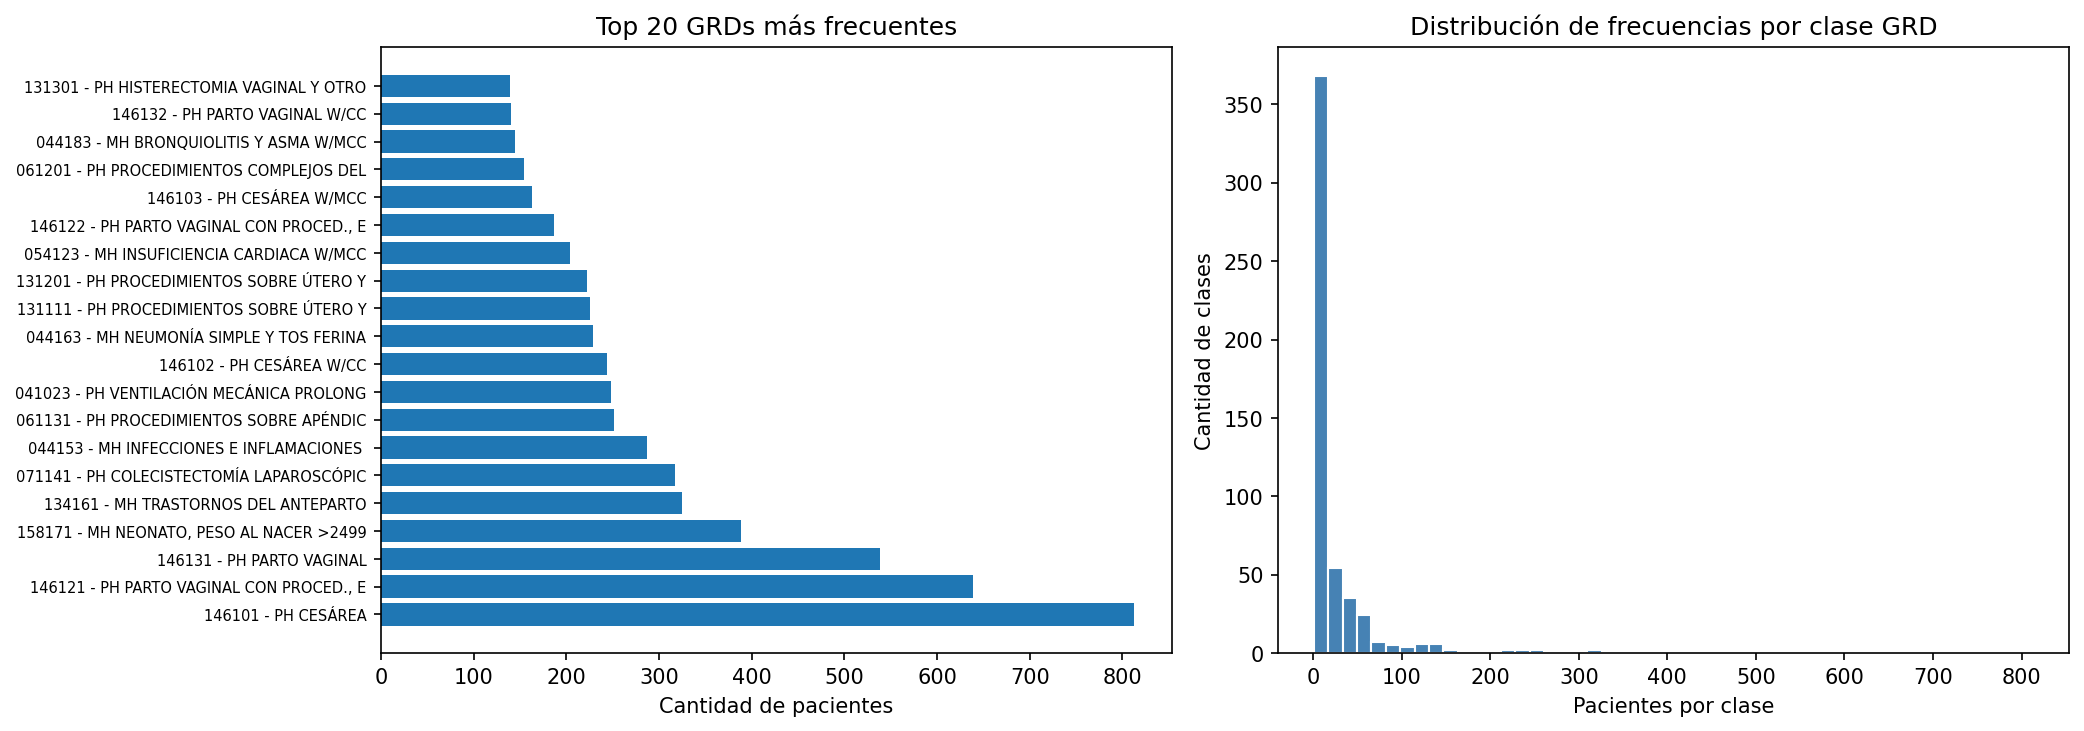
\includegraphics[width=\columnwidth]{grd_distribucion.png}
  \caption{Distribution of the top-20 most frequent GRD classes.}
  \label{fig:grd_dist}
\end{figure}

\textbf{Demographics overview.}
Age distribution and sex breakdown are visualised in
Fig.~\ref{fig:demographics}.

\begin{figure}[H]
  \centering
  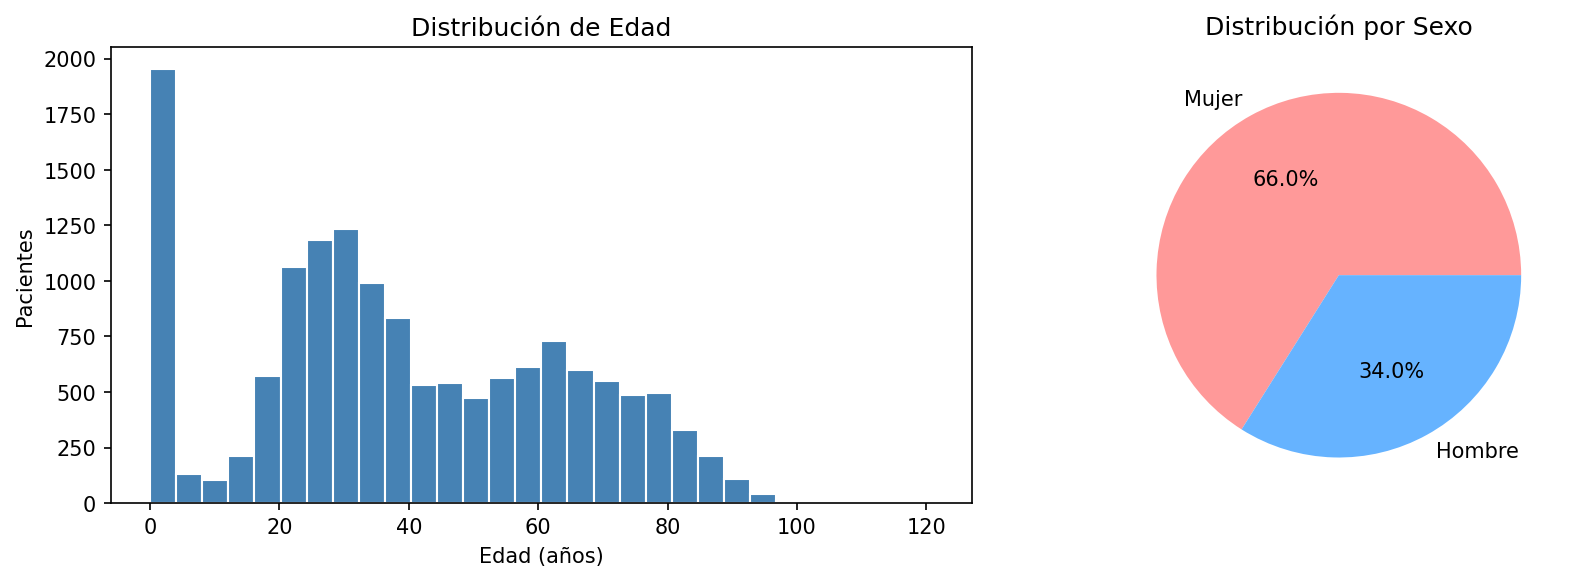
\includegraphics[width=\columnwidth]{demograficos.png}
  \caption{Patient age and sex distribution.}
  \label{fig:demographics}
\end{figure}

\textbf{Diagnoses and procedures per patient.}
On average, each patient record includes the full complement of
diagnosis and procedure fields provided by the hospital's
information system.
Fig.~\ref{fig:diag_proc} shows the distribution of populated fields.

\begin{figure}[H]
  \centering
  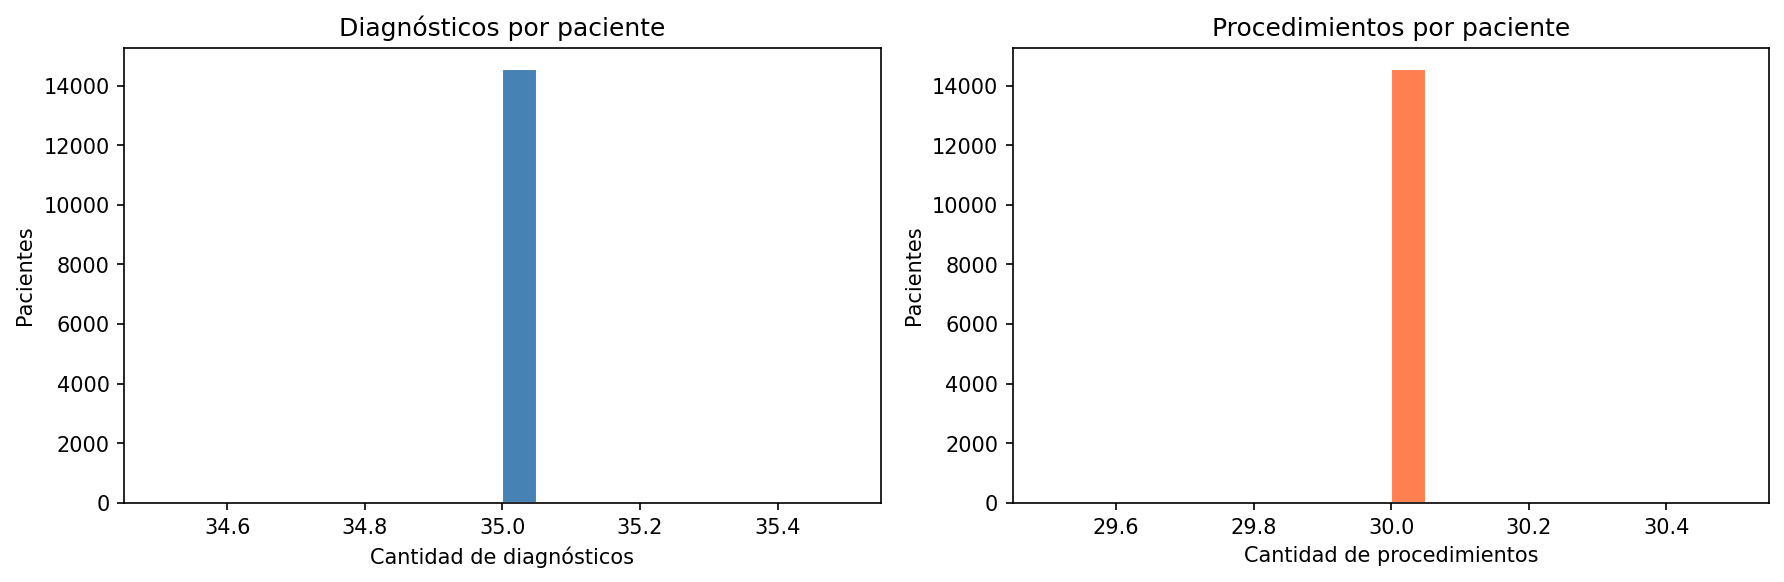
\includegraphics[width=\columnwidth]{diag_proced_por_paciente.png}
  \caption{Number of diagnoses and procedures per patient.}
  \label{fig:diag_proc}
\end{figure}

% ── 6. Experiments ──────────────────────────────────────────
\section{Experiments}

\subsection{Feature Justification}

The choice of top-$k$ multi-hot ICD encoding is motivated by two
constraints: (1) the ICD codes are the primary clinical signal
linking patient episodes to DRG groups by definition~\cite{fetter1980drg};
(2) we deliberately avoid free-text fields to keep the pipeline
deployable in hospitals without NLP infrastructure.
The vocabulary sizes (top-200 diagnoses, top-83 procedures) were
selected to cover $>95\%$ of code occurrences in the training set
while keeping the feature space tractable (287 dimensions).

\subsection{Results and Discussion}

Table~\ref{tab:results} reports performance on the validation set.

\begin{table}[H]
  \centering
  \caption{Model Performance on Validation Set (230 classes)}
  \label{tab:results}
  \begin{tabular}{lcccc}
    \toprule
    Model & Acc & Mac-F1 & W-F1 & Top-3 \\
    \midrule
    Random Forest  & 0.504 & 0.165 & 0.426 & 0.761 \\
    LightGBM       & 0.461 & 0.292 & 0.475 & 0.636 \\
    \textbf{MLP}   & \textbf{0.638} & \textbf{0.420}
                   & \textbf{0.617} & \textbf{0.842} \\
    \bottomrule
  \end{tabular}
\end{table}

The MLP dominates on all four metrics.
Notably, its Top-3 Accuracy of 84.2\% indicates that the correct
DRG is almost always within the model's top three predictions,
which is clinically meaningful: a decision-support tool presenting
three candidate DRGs would resolve the correct assignment in 84\%
of cases.

LightGBM achieves the best Macro-F1 among tree-based methods
(0.292), reflecting superior handling of minority classes
through its gradient-boosting objective.
Random Forest obtains a higher accuracy than LightGBM (0.504 vs
0.461) but a much lower Macro-F1 (0.165), suggesting it
heavily favours the majority classes.

Fig.~\ref{fig:comparison} visualises the three metrics per model.

\begin{figure}[H]
  \centering
  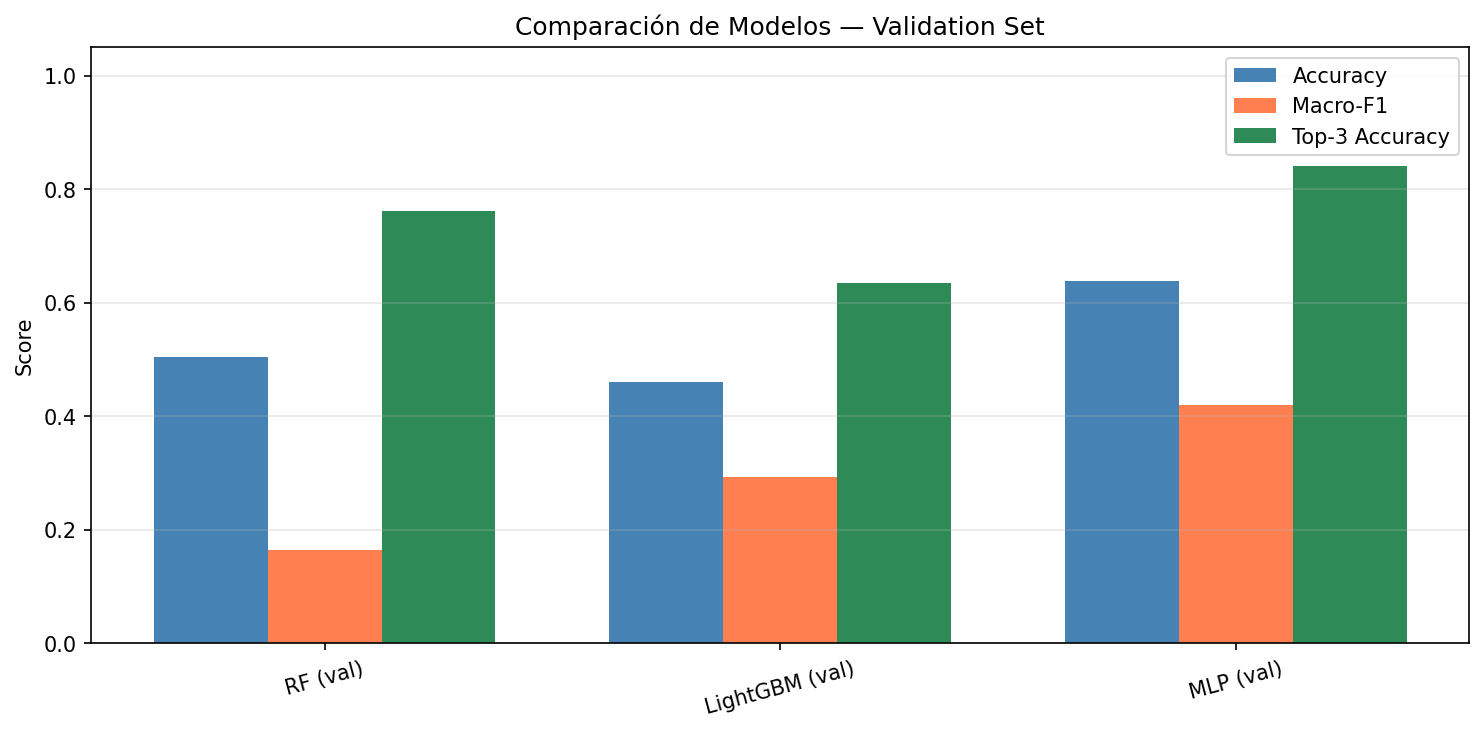
\includegraphics[width=\columnwidth]{comparacion_modelos.png}
  \caption{Metric comparison across models on the validation set.}
  \label{fig:comparison}
\end{figure}

\subsection{MLP Architecture and Training}

The selected MLP architecture is described in
Table~\ref{tab:arch}.
The three hidden layers progressively compress the 287-dimensional
input to a 128-dimensional representation before the 230-class
softmax output.
Batch Normalisation stabilises training, while Dropout prevents
co-adaptation of neurons.

\begin{table}[H]
  \centering
  \caption{MLP Architecture}
  \label{tab:arch}
  \begin{tabular}{lcc}
    \toprule
    Layer & Units & Extras \\
    \midrule
    Input         & 287   & –  \\
    Dense (ReLU)  & 512   & BatchNorm, Dropout 0.4 \\
    Dense (ReLU)  & 256   & BatchNorm, Dropout 0.3 \\
    Dense (ReLU)  & 128   & Dropout 0.2 \\
    Output (Softmax) & 230 & – \\
    \bottomrule
  \end{tabular}
\end{table}

The model converges in approximately 35 epochs with EarlyStopping
(patience 10).
Fig.~\ref{fig:curves} shows the learning curves.
A moderate overfitting gap is visible (train accuracy $\approx$83\%,
val accuracy $\approx$64\%), confirming that the model has sufficient
capacity and that the main limitation is data volume for the
long-tail classes.

\begin{figure}[H]
  \centering
  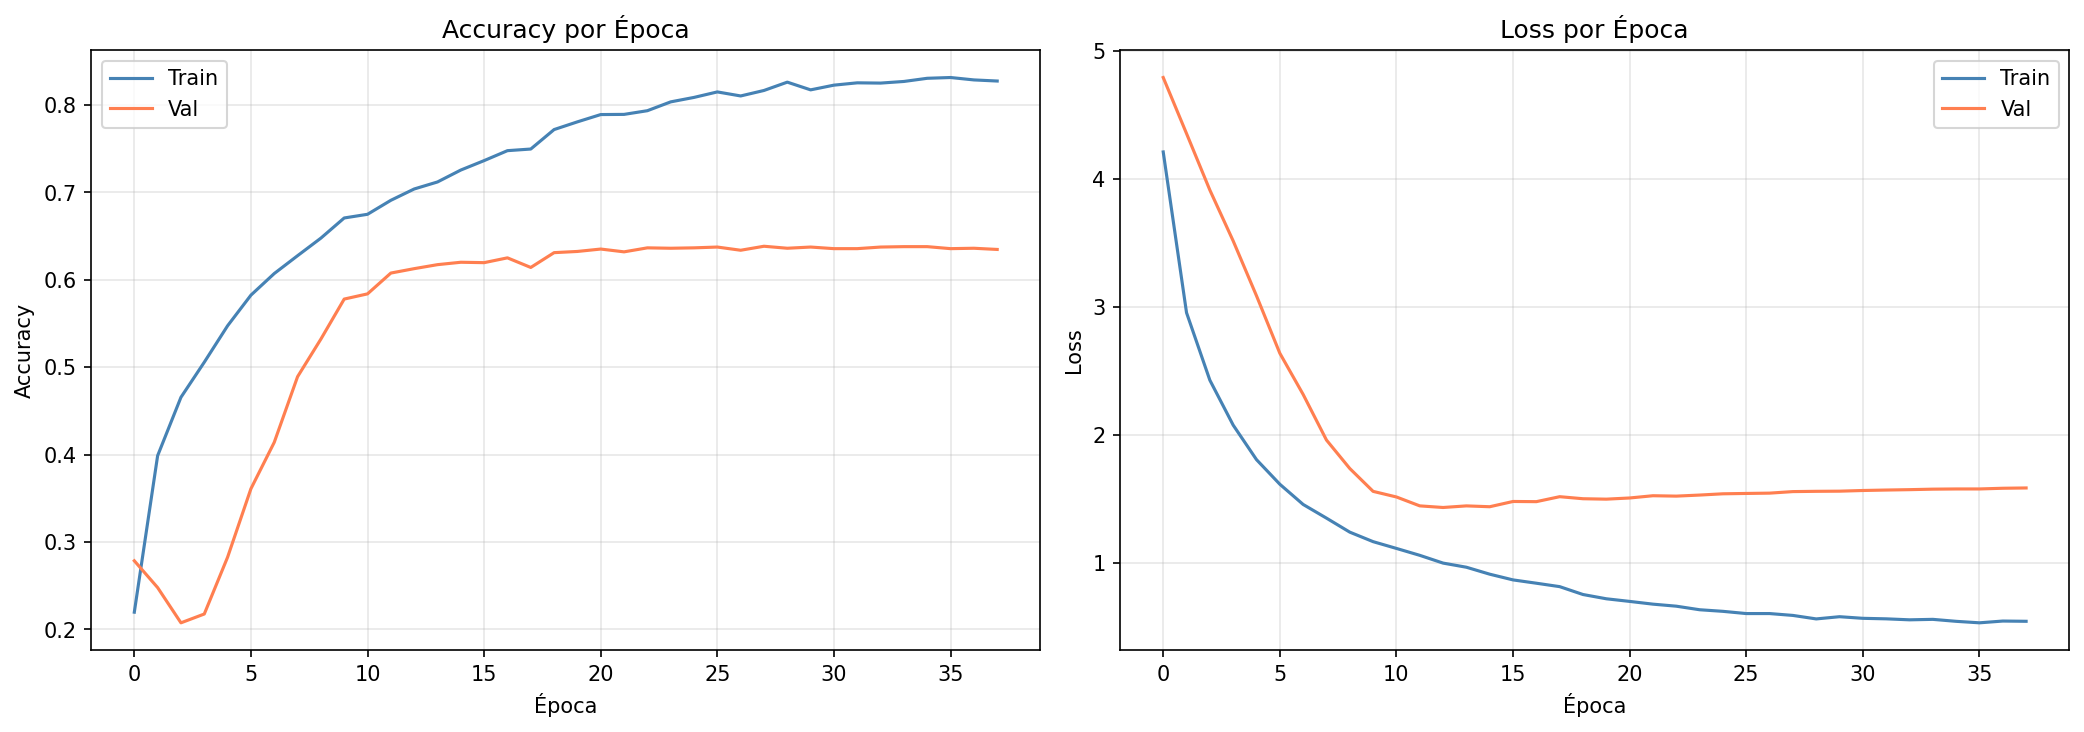
\includegraphics[width=\columnwidth]{curvas_entrenamiento_mlp.png}
  \caption{MLP training and validation learning curves.}
  \label{fig:curves}
\end{figure}

\subsection{Error Analysis}

Fig.~\ref{fig:cm} shows the normalised confusion matrix restricted
to the 15 most frequent GRD classes.
Most high-frequency DRGs are classified with $\geq 93\%$ per-class
accuracy.
The main source of confusion is between \texttt{146101}
(Vaginal delivery, MCC/CC absent) and \texttt{146102}
(Vaginal delivery, without MCC/CC): only 61\% of \texttt{146102}
episodes are correctly identified; 39\% are misclassified as
\texttt{146101}.
This is expected—the two codes differ only in complication or
comorbidity flags that may not be consistently coded in secondary
diagnoses.

\begin{figure}[H]
  \centering
  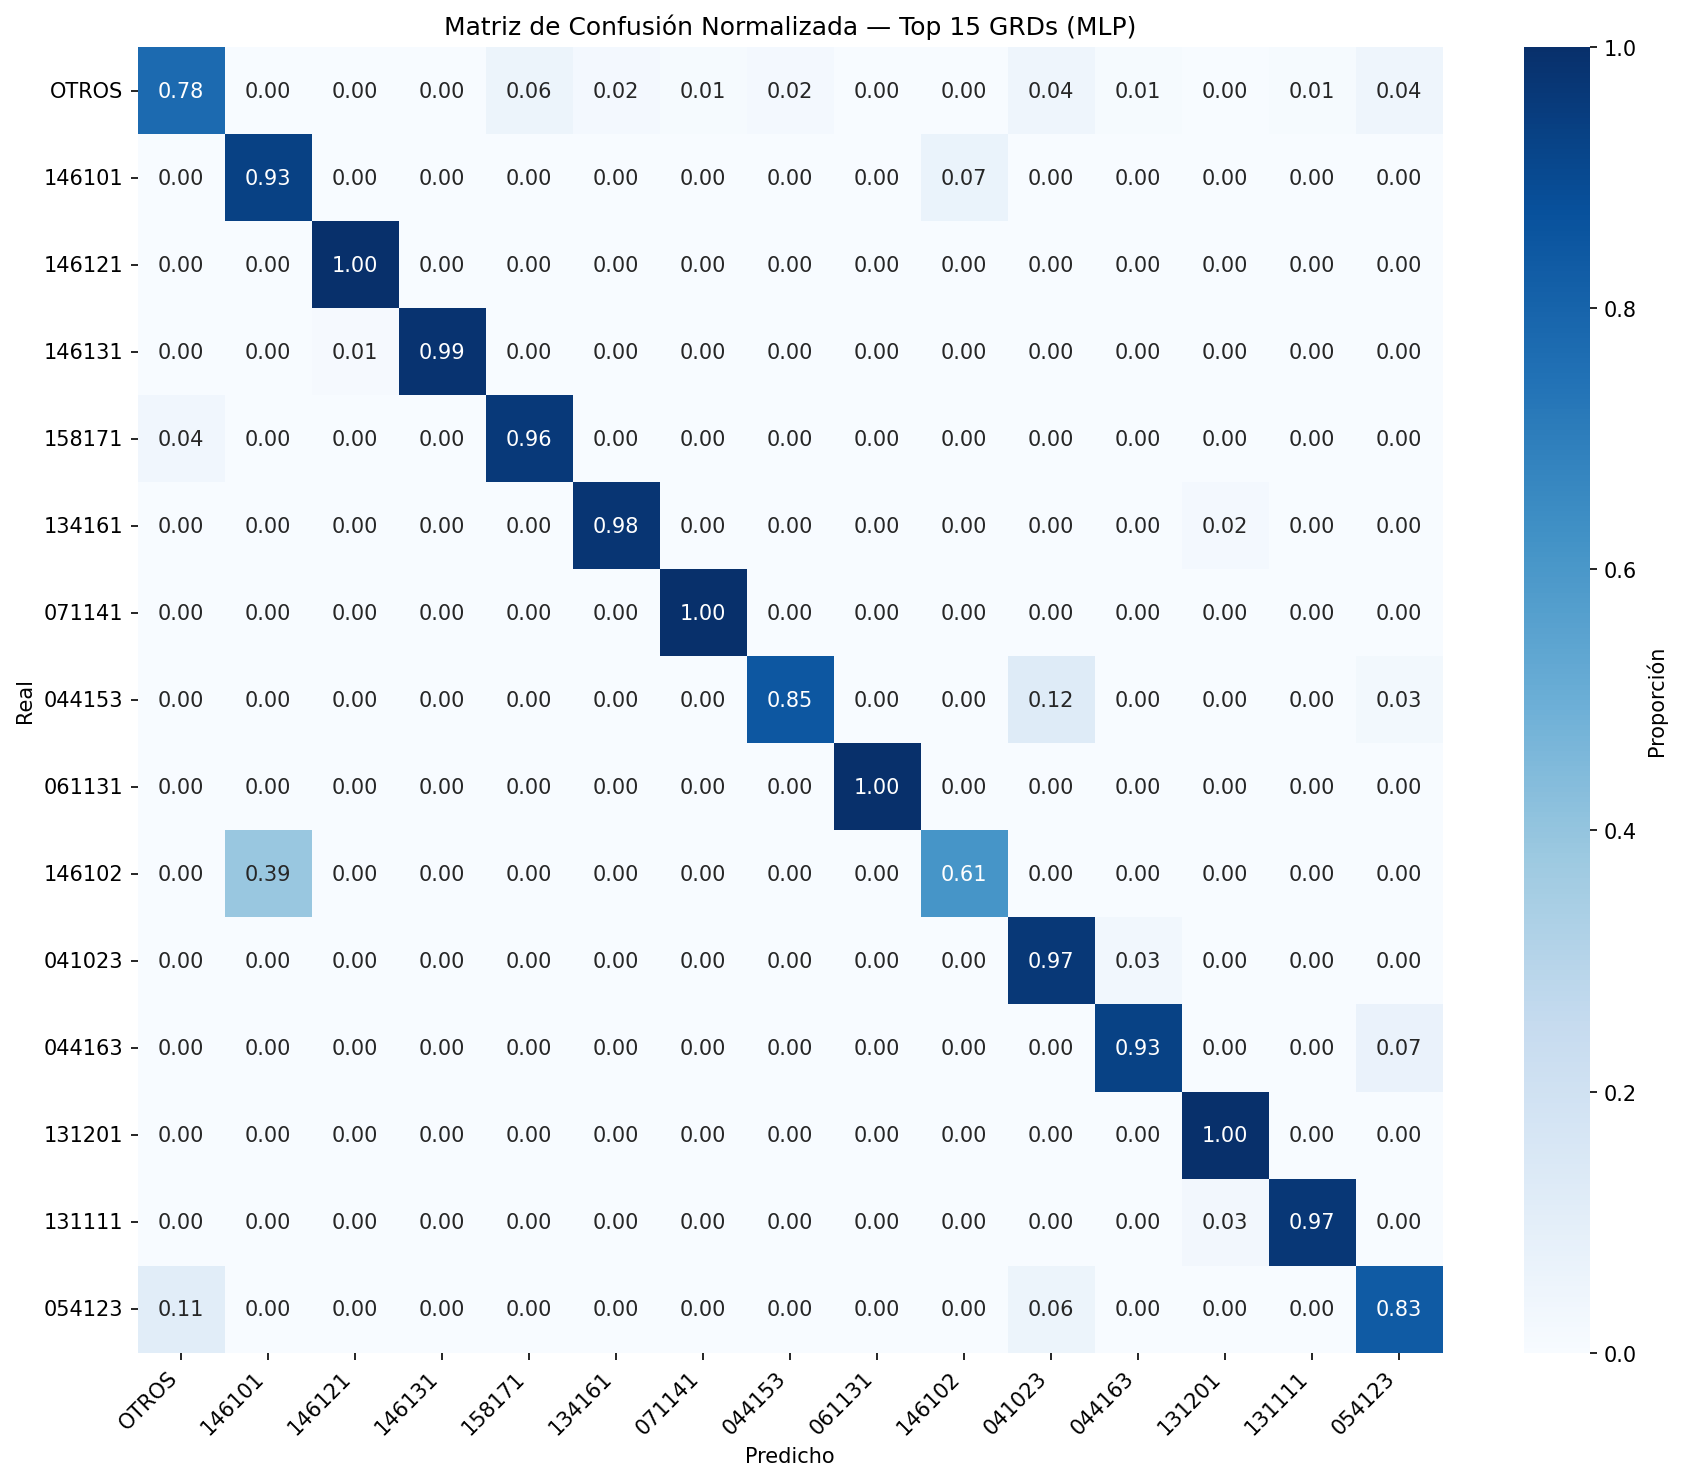
\includegraphics[width=\columnwidth]{confusion_matrix_top15.png}
  \caption{Normalised confusion matrix for the MLP on the top-15
           GRD classes (test set).}
  \label{fig:cm}
\end{figure}

\subsection{Comparison with Related Work}

Table~\ref{tab:comparison} contextualises our results against
the literature.
Direct comparison is hampered by differences in DRG nomenclature,
dataset size, and class granularity; nonetheless, our results
are consistent with the general findings: neural networks
outperform classical ensembles, and top-$k$ accuracy is
substantially higher than top-1 for DRG-level prediction.

\begin{table}[H]
  \centering
  \caption{Comparison with Related Work}
  \label{tab:comparison}
  \begin{tabular}{lccc}
    \toprule
    Work & Classes & Method & Accuracy \\
    \midrule
    Raju et al.~\cite{raju2021drg} & 25 (MDC) & GBDT & 0.72 \\
    Goldstein et al.~\cite{goldstein2016machine} & 30 & RF & 0.68 \\
    \textbf{This work} & \textbf{230} & \textbf{MLP} & \textbf{0.638} \\
    \bottomrule
  \end{tabular}
\end{table}

Our accuracy of 63.8\% at 230-class granularity is competitive:
Raju et al.~achieve 72\% but on only 25 Major Diagnostic Categories,
a much easier task.
Goldstein et al.~report 68\% with 30 classes.
The fact that we operate at 230 classes with a small-to-medium
dataset (14k patients) underlines the difficulty of the task
and the strength of our multiclass MLP approach.

% ── 7. Conclusions ──────────────────────────────────────────
\section{Conclusions}

We presented a complete machine learning pipeline for automatic
DRG prediction from structured clinical data at Hospital El Pino.
Our key findings are:

\begin{enumerate}
  \item \textbf{Long-tail strategy is effective.}
        Grouping DRGs with fewer than 10 examples into
        \textsc{Others} retains 92.4\% of the data specificity
        while reducing the target space from 526 to 230 classes,
        making the problem tractable for all three models.

  \item \textbf{MLP outperforms tree-based models.}
        With 63.8\% accuracy, 42.0\% macro-F1, and 84.2\%
        top-3 accuracy on validation, the MLP is the strongest
        model and is particularly suitable for a clinical
        decision-support setting where presenting three candidate
        DRGs is acceptable.

  \item \textbf{Severity-level confusion is the main error source.}
        The most frequent misclassications occur between DRGs
        that share the base code but differ in severity suffix
        (e.g., 146101 vs 146102), a challenge inherent to the
        IR-GRD coding logic.
\end{enumerate}

% ── 8. Limitations and Future Work ──────────────────────────
\section{Limitations and Future Work}

\textbf{Limitations.}
The dataset is limited to 14{,}561 records from a single hospital,
which restricts generalisability.
The moderate overfitting gap (83\% train vs 64\% val accuracy)
suggests that a larger corpus would benefit the MLP.
Furthermore, our feature engineering discards the free-text
descriptions embedded in the ICD strings, likely losing
clinical nuance.

\textbf{Future Work.}
\begin{itemize}
  \item \textit{Class-weighted training.}
        Applying inverse-frequency weights to the loss function
        may improve Macro-F1 for minority DRGs without discarding
        data.
  \item \textit{Embedding-based encoding.}
        Replacing multi-hot with pre-trained ICD embeddings
        (e.g., Med2Vec~\cite{choi2016m2v}) could capture
        semantic relatedness between codes.
  \item \textit{Multi-hospital generalisation.}
        Training on data from multiple hospitals and validating
        cross-site is necessary for production deployment.
  \item \textit{Severity prediction cascade.}
        A two-stage pipeline—first predict DRG base, then
        predict severity—could reduce the most frequent
        confusion errors.
  \item \textit{Explainability.}
        SHAP analysis on the MLP outputs would make the model
        auditable by clinical coders.
\end{itemize}

% ── Bibliography ────────────────────────────────────────────
\begin{thebibliography}{00}

\bibitem{fetter1980drg}
R.~B. Fetter, Y.~Shin, J.~L. Freeman, R.~F. Averill, and J.~D. Thompson,
``Case mix definition by diagnosis-related groups,''
\textit{Medical Care}, vol.~18, no.~2, pp.~iii--53, 1980.

\bibitem{topol2019highperformance}
E.~J. Topol,
``High-performance medicine: the convergence of human and artificial
intelligence,''
\textit{Nature Medicine}, vol.~25, no.~1, pp.~44--56, 2019.

\bibitem{mullenbach2018explainable}
J.~Mullenbach, S.~Wiegreffe, J.~Duke, J.~Sun, and J.~Eisenstein,
``Explainable prediction of medical codes from clinical text,''
in \textit{Proc. NAACL-HLT}, New Orleans, LA, 2018, pp.~1101--1111.

\bibitem{huang2019clinicalbert}
K.~Huang, J.~Altosaar, and R.~Ranganath,
``ClinicalBERT: Modeling clinical notes and predicting hospital
readmission,''
\textit{arXiv preprint arXiv:1904.05342}, 2019.

\bibitem{raju2021drg}
B.~Raju, F.~Martinot-Lagarde, and T.~Le,
``DRG prediction using gradient boosted decision trees on
structured EHR data,''
in \textit{Proc. AMIA Annual Symposium}, 2021, pp.~1013--1022.

\bibitem{chawla2002smote}
N.~V. Chawla, K.~W. Bowyer, L.~O. Hall, and W.~P. Kegelmeyer,
``SMOTE: Synthetic minority over-sampling technique,''
\textit{Journal of Artificial Intelligence Research},
vol.~16, pp.~321--357, 2002.

\bibitem{chen2019hiagm}
H.~Chen, X.~Ma, Z.~Lin, J.~Ding, P.~Wei, H.~Liu, and H.~Chen,
``Hierarchical text classification with multi-label representation
learning,''
in \textit{Proc. CIKM}, 2019, pp.~2841--2849.

\bibitem{purushotham2018benchmarking}
S.~Purushotham, C.~Meng, Z.~Che, and Y.~Liu,
``Benchmarking deep learning models on MIMIC-III,''
\textit{Journal of Biomedical Informatics}, vol.~83, pp.~112--134, 2018.

\bibitem{ke2017lightgbm}
G.~Ke, Q.~Meng, T.~Finley, T.~Wang, W.~Chen, W.~Ma, Q.~Ye, and T.~Y. Liu,
``LightGBM: A highly efficient gradient boosting decision tree,''
in \textit{Proc. NeurIPS}, Long Beach, CA, 2017, pp.~3146--3154.

\bibitem{goldstein2016machine}
B.~A. Goldstein, A.~M. Navar, M.~J. Pencina, and J.~P.~A. Ioannidis,
``Opportunities and challenges in developing risk prediction models with
electronic health records data,''
\textit{Journal of the American Medical Informatics Association},
vol.~24, no.~1, pp.~198--208, 2017.

\bibitem{choi2016m2v}
E.~Choi, M.~T. Bahadori, E.~Searles, C.~Coffey, M.~Thompson,
J.~Bost, J.~Tejedor-Sojo, and J.~Sun,
``Multi-layer representation learning for medical concepts,''
in \textit{Proc. KDD}, San Francisco, CA, 2016, pp.~1495--1504.

\end{thebibliography}

\end{document}
